%%%%%%%%%%%%%%%%%%%%%%%%%%%%%%%%%%%%%%%
% Wenneker Resume/CV
% LaTeX Template
% Version 1.1 (19/6/2016)
%
% This template has been downloaded from:
% http://www.LaTeXTemplates.com
%
% Original author:
% Frits Wenneker (http://www.howtotex.com) with extensive modifications by 
% Vel (vel@LaTeXTemplates.com)
%
% License:
% CC BY-NC-SA 3.0 (http://creativecommons.org/licenses/by-nc-sa/3.0/
%
%%%%%%%%%%%%%%%%%%%%%%%%%%%%%%%%%%%%%%

%----------------------------------------------------------------------------------------
%	PACKAGES AND OTHER DOCUMENT CONFIGURATIONS
%----------------------------------------------------------------------------------------

\documentclass[a4paper,10pt]{memoir} % Font and paper size

%%%%%%%%%%%%%%%%%%%%%%%%%%%%%%%%%%%%%%%%%
% Wenneker Resume/CV
% Structure Specification File
% Version 1.1 (19/6/2016)
%
% This file has been downloaded from:
% http://www.LaTeXTemplates.com
%
% Original author:
% Frits Wenneker (http://www.howtotex.com) with extensive modifications by 
% Vel (vel@latextemplates.com)
%
% License:
% CC BY-NC-SA 3.0 (http://creativecommons.org/licenses/by-nc-sa/3.0/)
%
%%%%%%%%%%%%%%%%%%%%%%%%%%%%%%%%%%%%%%%%%

%----------------------------------------------------------------------------------------
%	PACKAGES AND OTHER DOCUMENT CONFIGURATIONS
%----------------------------------------------------------------------------------------

\usepackage{XCharter} % Use the Bitstream Charter font
\usepackage[utf8]{inputenc} % Required for inputting international characters
\usepackage[T1]{fontenc} % Output font encoding for international characters

\usepackage[top=1cm,left=1cm,right=1cm,bottom=1cm]{geometry} % Modify margins

\usepackage{graphicx} % Required for figures

\usepackage{flowfram} % Required for the multi-column layout

\usepackage{url} % URLs

\usepackage[usenames,dvipsnames,table]{xcolor} % Required for custom colours

\usepackage{tikz} % Required for the horizontal rule

\usepackage{enumitem} % Required for modifying lists
\setlist{noitemsep,nolistsep} % Remove spacing within and around lists

\setlength{\columnsep}{\baselineskip} % Set the spacing between columns

% Define the left frame (sidebar)
\newflowframe{0.2\textwidth}{\textheight}{0pt}{0pt}[left]
\newlength{\LeftMainSep}
\setlength{\LeftMainSep}{0.2\textwidth}
\addtolength{\LeftMainSep}{1\columnsep}
 
% Small static frame for the vertical line
\newstaticframe{1.5pt}{\textheight}{\LeftMainSep}{0pt}
 
% Content of the static frame with the vertical line
\begin{staticcontents}{1}
\hfill
\tikz{\draw[loosely dotted,color=RoyalBlue,line width=1.5pt,yshift=0](0,0) -- (0,\textheight);}
\hfill\mbox{}
\end{staticcontents}
 
% Define the right frame (main body)
\addtolength{\LeftMainSep}{1.5pt}
\addtolength{\LeftMainSep}{1\columnsep}
\newflowframe{0.7\textwidth}{\textheight}{\LeftMainSep}{0pt}[main01]

\pagestyle{empty} % Disable all page numbering

\setlength{\parindent}{0pt} % Stop paragraph indentation

%----------------------------------------------------------------------------------------
%	NEW COMMANDS
%----------------------------------------------------------------------------------------

\newcommand{\userinformation}[1]{\renewcommand{\userinformation}{#1}} % Define a new command for the CV user's information that goes into the left column

\newcommand{\cvheading}[1]{{\Huge\bfseries\color{RoyalBlue} #1} \par\vspace{.6\baselineskip}} % New command for the CV heading
\newcommand{\cvsubheading}[1]{{\Large\bfseries #1} \bigbreak} % New command for the CV subheading

\newcommand{\Sep}{\vspace{1em}} % New command for the spacing between headings
\newcommand{\SmallSep}{\vspace{0.5em}} % New command for the spacing within headings

\newcommand{\aboutme}[2]{ % New command for the about me section
\textbf{\color{RoyalBlue} #1}~~#2\par\Sep
}
	
\newcommand{\CVSection}[1]{ % New command for the headings within sections
{\Large\textbf{#1}}\par
\SmallSep % Used for spacing
}

\newcommand{\CVItem}[2]{ % New command for the item descriptions
\textbf{\color{RoyalBlue} #1}\par
#2
\SmallSep % Used for spacing
}

\newcommand{\bluebullet}{\textcolor{RoyalBlue}{$\circ$}~~} % New command for the blue bullets
 % Include the file specifying document layout and packages

\usepackage{tabularx}
\usepackage{multirow}
\usepackage[table]{xcolor}

\definecolor{darkergray}{HTML}{EEEEEE}
\definecolor{lightergray}{HTML}{FAFAFA}
\definecolor{linkblue}{HTML}{337AB7}

\rowcolors{0}{darkergray}{lightergray}

%----------------------------------------------------------------------------------------
%	NAME AND CONTACT INFORMATION 
%----------------------------------------------------------------------------------------

\userinformation{ % Set the content that goes into the sidebar of each page
\begin{flushright}
% Comment out this figure block if you don't want a photo
% 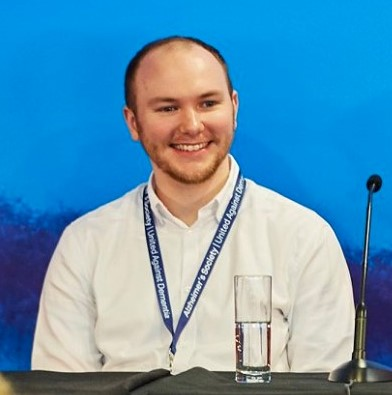
\includegraphics[width=0.6\columnwidth]{profilepic.jpg}\\[\baselineskip] % Your photo
\small % Smaller font size
Luke Tait \\ % Your name
\scriptsize
\url{taitl2@cardiff.ac.uk} \\ % Your email address
\url{lukewtait.github.io} \\ % Your URL
% (000) 111-1111 \\ % Your phone number
\Sep % Some whitespace
\small
\textbf{Address} \\
CUBRIC \\ % Address 1
Maindy Road \\
Cardiff \\ % Address 2
CF24 4HQ \\ % Address 3
\vfill % Whitespace under this block to push it up under the photo
\end{flushright}
}

%----------------------------------------------------------------------------------------

\begin{document}

\begin{flushright}
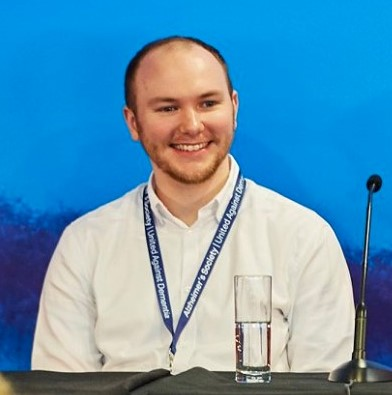
\includegraphics[width=0.6\columnwidth]{profilepic.jpg}\\[\baselineskip] % Your photo
\end{flushright}
\userinformation % Print your information in the left column

\framebreak % End of the first column

%----------------------------------------------------------------------------------------
%	HEADING
%----------------------------------------------------------------------------------------

\cvheading{Luke Tait} % Large heading - your name

\cvsubheading{PhD} % Subheading - your occupation/specialization

%----------------------------------------------------------------------------------------
%	ABOUT ME
%----------------------------------------------------------------------------------------

\aboutme{Research}{My research interests invole the use of computational techniques such as time series analysis, graph theory, and non-linear dynamical systems to understand brain dynamics during cognitive processes and in neurodegenerative disorders. I joined the Cardiff University Brain Research Imaging Centre in July 2019 as a Research Associate in Dr Jiaxiang Zhang's lab, integrating functional imaging (fMRI, MEG) and computational modelling to understand the neuronal mechanisms underpinning decision making. Prior to this, the focus of my PhD research was using similar techniques to understand alterations to brain dynamics in Alzheimer’s disease. }

%----------------------------------------------------------------------------------------
%	EXPERIENCE
%----------------------------------------------------------------------------------------

\CVSection{Research Positions}

%------------------------------------------------

\CVItem{July 2019 - present, \textit{Research Associate}, Cardiff University}{
Post-doctoral research with Dr Jiaxiang Zhang and the Cognition and Computational Brain Lab at Cardiff University Brain Research Imaging Centre. Using computational techniques to study the neuronal mechanisms underpinning cognitive processes such as perceptual decision making. 
}

%------------------------------------------------

%----------------------------------------------------------------------------------------
%	EDUCATION
%----------------------------------------------------------------------------------------

\CVSection{Education}

%------------------------------------------------

\CVItem{2015 - 2019, Univeristy of Exeter (Alzheimer's Society Doctoral Training Centre)}{
\textbf{Multi-scale Mathematical Modelling of Brain Networks in Alzheimer's Disease}\\
\textit{Supervisors:} Dr Marc Goodfellow (Mathematics), Dr Jon T Brown (Medical School) \\
The primary focus during my PhD was on characterising and modelling alterations to brain dynamics in Alzheimer’s disease in order to gain mechanistic insight into the relationship between pathology, function, and phenotype. This work ranged from dynamics of individual or local networks of neurons in animal models of dementia pathologies, to whole brain oscillatory dynamics recorded by EEG. During my PhD, I developed tools to study EEG microstates of the brain as a biomarker to aid with early diagnosis of Alzheimer's disease. This work additionally included a three month secondment from seed-corn funding modelling neuronal dynamics in the spatial navigation systems of the brain. 
}

%------------------------------------------------

\CVItem{2011 - 2015, \textit{MMath Mathematical Physics}, University of Liverpool}{
First Class Honours\\
%Dissertations: 
%\begin{itemize}
%\item An Analysis of a String Model in the Free Fermionic Formulation. Supervisor: Prof. Alon Faraggi.
%\item The Multipole Method of Solving Laplace’s Equation in Two Dimensions. Supervisor: Dr Ian Thompson.
%\end{itemize}
%Awards:
%\begin{itemize}
%\item NA Software Honours Prize for Best Project in the Field of Mathematical Software
%\end{itemize}
}

\Sep % Extra whitespace after the end of a major section

%----------------------------------------------------------------------------------------
%	KEY SKILLS
%----------------------------------------------------------------------------------------

\CVSection{Key Skills}

%------------------------------------------------

\CVItem{Programming}{I am an experienced user of Matlab, and also have experience with Python, R, and Maple. This has predominantly been applied to computational data analysis, statistical techniques, and numerical simulations.}

%------------------------------------------------

\CVItem{Mathematical expertise}{Time series analysis, graph theory, bifurcation theory & dynamical systems, numerical/ computational modelling, statistical analysis, model parameter fitting, inverse problems. Multi-scaled brain modelling including biophysical and phenomenological point neuron models, neuronal network models, neural mass/field models, and coupled oscillators.}

%------------------------------------------------

\CVItem{Neuroimaging}{My primary area of expertise is non-invasive human neuroimaging such as EEG, MEG, MRI, and fMRI. I am experienced with software such as Fieldtrip, Brainstorm, SPM, and Freesurfer for analysis of these data. I additionally have experience working with two-photon calcium imaging data in rodents, and spent six months performing whole cell patch clamp experiments from slice.}

\Sep % Extra whitespace after the end of a major section

%----------------------------------------------------------------------------------------
%	FUNDING AND AWARDS
%----------------------------------------------------------------------------------------

\CVSection{Funding and Awards}

%------------------------------------------------

\CVItem{Travel Grant}{Guarantors of Brain, £600}

%------------------------------------------------

\CVItem{NA Software Honours Prize for Best Project in the Field of Mathematical Software}{Awarded for my undergraduate dissertation.}

%------------------------------------------------

\Sep % Extra whitespace after the end of a major section

%----------------------------------------------------------------------------------------
%	NEW PAGE DELIMITER
%	Place this block wherever you would like the content of your CV to go onto the next page
%----------------------------------------------------------------------------------------

\clearpage % Start a new page

\userinformation % Print your information in the left column

\framebreak % End of the first column

%----------------------------------------------------------------------------------------
%	PUBLICATIONS AND PRESENTATIONS
%----------------------------------------------------------------------------------------

\CVSection{Publications and Presentations}

%------------------------------------------------

\CVItem{Preprints}{
\begin{tabular}{p{0.96\columnwidth}}
\textcolor{linkblue}{Cortical source imaging of resting-state MEG with a high resolution atlas: An evaluation of methods} \newline
\textbf{Tait L}, Ozkan A, Szul MJ, Zhang J \newline
bioRxiv 2020.01.12.903302 (2020) \\

\textcolor{linkblue}{EEG microstate complexity for aiding early diagnosis of Alzheimer's disease} \newline
\textbf{Tait L}, Tamagnini F, Stothart G, Barvas E, Monaldini C, Frusciante R, Volpini M, Guttmann S, Coulthard E, Brown JT, Kazanina N, Goodfellow M \newline
 bioRxiv 833244 (2019) 
\end{tabular}
}

\CVItem{Journal Articles}{
\begin{tabular}{p{0.96\columnwidth}}
\textcolor{linkblue}{Computational modelling in source space from scalp EEG to inform presurgical evaluation of epilepsy surgery} \newline
Lopes M, Junges L, \textbf{Tait L}, Terry JR, Abela E, Richardson MP, Goodfellow M \newline
Clinical Neurophysiology 131(1):225-234 (2020) \\

\textcolor{linkblue}{Network Substrates of Cognitive Impairment in Alzheimer's Disease} \newline
\textbf{Tait L}, Stothart G, Coulthard E, Brown JT, Kazanina N, Goodfellow M \newline
 Clinical Neurophysiology 130(9):1581-1595 (2019) \\

\textcolor{linkblue}{Control of clustered action potential firing in a mathematical model of entorhinal cortex stellate cells} \newline
\textbf{Tait L}, Wedgwood K, Tsaneva-Atanasova K, Brown JT, Goodfellow M \newline
 Journal of Theoretical Biology 449:23-34 (2018) 

\end{tabular}
}

\CVItem{Conference Proceedings}{
\begin{tabular}{p{0.96\columnwidth}}
\textcolor{linkblue}{Graph-theoretical measures provide translational markers of large-scale brain network disruption in human dementia patients and animal models of dementia} \newline
Stothart G, Petkov G, Kazanina N, Goodfellow M, \textbf{Tait L}, Brown JT\newline
International Journal of Psychophysiology 108:71  (2016)
\end{tabular}
}

\CVItem{Oral Presentations}{
\begin{tabular}{p{0.96\columnwidth}}
\textcolor{linkblue}{AlzSM: Using EEG to understand Alzheimer’s disease and develop biomarkers}. Alzheimer's Society Annual Conference, London, May 2019. \\
\textcolor{linkblue}{Analysis of the EEG of Alzheimer’s Patients}. Computational Biology Symposium, University of Exeter, July 2018. \\
\textcolor{linkblue}{Control of Clustered Action Potential Firing in a Mathematical Model of Entorhinal Cortex Stellate Cells}. Alzheimer’s Research UK South West and Wales Scientific Network Meeting, Bristol, May 2018. \\
\textcolor{linkblue}{Multi-scale functional network dysfunction in dementia}. Computational Biology Symposium, University of Exeter, June 2017. \\
\textcolor{linkblue}{Reduced Frontal Lobe Delta Power and Increased Network Homogeneity in a Mouse Model of Frontotemporal Dementia}. Network Biology Symposium, University of Exeter, June 2016. \\
\textcolor{linkblue}{Increased Network Homogeneity and Reduced Frontal Lobe Delta Power in a Mouse Model of Frontotemporal Dementia}. Alzheimer’s Research UK Annual Conference PhD Day, March 2016. 
\end{tabular}
}

\CVItem{Poster Presentations}{ 
\begin{tabular}{p{0.96\columnwidth}}
\textcolor{linkblue}{Control of Clustered Action Potential Firing in a Mathematical Model of Entorhinal Cortex Stellate Cells}. International Conference on Mathematical Neuroscience, Juan-les-Pins, France, June 2018. \\
\textcolor{linkblue}{Control of Clustered Action Potential Firing in a Mathematical Model of Entorhinal Cortex Stellate Cells}. Alzheimer’s Research UK South West and Wales Scientific Network Meeting. Bristol, May 2018. \\ 
\textcolor{linkblue}{Control of Clustered Action Potential Firing in a Mathematical Model of Entorhinal Cortex Stellate Cells}. Brain Networks and Neurological Disorders: From Theory to Clinic, University of Exeter, UK, April 2018. \\
\textcolor{linkblue}{Decreased Delta Synchrony, Reduced Frontal Lobe Delta Power, and Increased Network Homogeneity in a Mouse Model of Frontotemporal Dementia}. Alzheimer’s Society Annual Conference, Bristol , UK, June 2016. \\
\textcolor{linkblue}{Increased Network Homogeneity and Reduced Frontal Lobe Delta Power in a Mouse Model of Frontotemporal Dementia}. Alzheimer’s Research UK Annual Conference, Manchester, UK, March 2016.
\end{tabular}
}


\Sep % Extra whitespace after the end of a major section

%----------------------------------------------------------------------------------------
%	NEW PAGE DELIMITER
%	Place this block wherever you would like the content of your CV to go onto the next page
%----------------------------------------------------------------------------------------

\clearpage % Start a new page

\userinformation % Print your information in the left column

\framebreak % End of the first column

%------------------------------------------------


%----------------------------------------------------------------------------------------
%	TEACHING
%----------------------------------------------------------------------------------------

\CVSection{Teaching}
\CVItem{Supervision}{ 
\bluebullet 2019-Present: Co-supervision of a PhD student at Reading University School of Pharmacology using EEG to aid with diagnosis of Alzheimer's disease\\
\bluebullet January-April 2019: Supervision of 4 month PhD training year project combining diffusion MRI data with whole brain computational models to test how structural connectivity reflects dynamics in memory disorders. \\
\bluebullet Summer 2018: Informal supervision of a 2nd year undergraduate summer project comparing 64 channel research grade and 14 channel “Emotiv” EEG headsets. \\
\bluebullet Summer 2018: Informal supervision of a M-level undergraduate summer project performing bifurcation analysis and numerical continuation of subthreshold oscillations and resonance in a neuronal model.
}

\CVItem{Demonstrating on undergraduate modules}{
\bluebullet Differential Equations: Responsibilities included planning and leading weekly additional support sessions for a small group (10 students) of 2nd year natural sciences students taking a course aimed at mathematics students. \\
\bluebullet Mathematics and Computing: Integrative Tools for Natural Sciences: I ran tutorial sessions on a range of topics in mathematics for 1st year natural sciences students.\\ 
\bluebullet Mathematical Modelling in Biology and Medicine: I assisted a series of lecturers in running tutorials for M level natural science students. 
}


%------------------------------------------------

\CVSection{Impact and Networking}

\CVItem{Conferences and Workshops Attended}{
\bluebullet Cognitive Computational Neuroscience, Berlin, German, September 2019.\\
\bluebullet Computational Biology Symposium, Exeter, UK, July 2018.\\
\bluebullet International Conference on Mathematical Neuroscience, Juan-les-Pines, France, June 2018.\\
\bluebullet Alzheimer’s Research UK South West and Wales Scientific Network Meeting, Bristol, May 2018. \\
\bluebullet BioDynamics. Royal College of Physicians, London, UK, April 2018. \\
\bluebullet Brain Networks and Neurological Disorders: from Theory to Clinic. Exeter, UK, April 2018. \\
\bluebullet Network Dynamics: Bridging Theoretical Advances and Applications. Exeter, UK,  April 2018. \\
\bluebullet Integrated Systems Neuroscience. Manchester, UK, September 2017. \\
\bluebullet Computational Biology Symposium, Exeter, June 2017.\\
\bluebullet Alzheimer’s Research UK Annual Conference. Aberdeen, UK, March 2017. \\
\bluebullet Alzheimer’s Research UK Annual Conference PhD Day. Aberdeen, UK, March 2017.\\
\bluebullet Symposia on Memory. Centre de Recerca Matematica, Barcelona, Spain, March 2017. \\
\bluebullet Computational Neurology. Newcastle, UK, February 2017. \\
\bluebullet Model Parameter Estimation for Predictive Medicine. Birmingham, UK, July 2016. \\
\bluebullet Alzheimer’s Society Annual Conference. Bristol, UK, June 2016. \\
\bluebullet Network Biology Symposium. Exeter, June 2016. \\
\bluebullet Alzheimer’s Research UK Annual Conference. Manchester, March 2016. \\
\bluebullet Alzheimer’s Research UK Annual Conference PhD Day. Manchester, March 2016. \\
\bluebullet Large Scale Brain Networks in Health and Disease: A GW4 Dissemination Event. M-Shed, Bristol. 8th Jan 2016. 
}

\CVItem{Public Engagement}{
\bluebullet Oral presentation at Alzheimer’s Research UK South-West public open day, Exeter, June 2018 \\
\bluebullet Stand at University of Exeter Public Engagement Day, Exeter, March 2018\\
\bluebullet Meet a Neuroscientist Event, Exeter, March 2018\\
\bluebullet Electrophysiology Stand at Brain Awareness Week Event to Schools, Exeter, March 2018\\
\bluebullet INSPIRE Lecture at Exeter Maths School, Exeter, December 2017\\
\bluebullet Stand at Alzheimer’s Society Memory Walk, Exeter, September 2017\\
\bluebullet Oral presentation at Alzheimer’s Society Legacy Fundraiser, Exeter, July 2017\\
\bluebullet Oral presentation at Exeter School, Exeter, March 2017\\
\bluebullet Stand at Alzheimer’s Society Memory Walk, Plymouth, October 2016\\
}



%------------------------------------------------

\Sep % Extra whitespace after the end of a major section

%----------------------------------------------------------------------------------------

\end{document}
